\subsection{Introduction to Quadrature}

\frame{
\frametitle{ We now approach the subject of numerical integration.}
\begin{block}{}
{\Huge The goal is to approximate the definite integral of $f(x)$ over the interval $[a, b]$ by evaluating $f(x)$ at a finite number of sample points. }
\end{block}
}

\frame{
\begin{block}{Definition 5.1.}
Suppose that $a = x_0 < x_1 < ··· < x_M = b$. 
A formula of the form 
\begin{equation*}
Q [f] = \sum_{k=0}^M w_k f(x_k) = w_0 f(x_0) + w_1 f(x_1) + \cdots + w_M f(x_M)
\end{equation*}
with the property that
\begin{equation*}
\int_a^b f(x) d x = Q [f] + E[f]
\end{equation*}
is called a numerical integration or quadrature formula. 
\begin{itemize}
\item The term $E[f]$ is called the truncation error for integration.  \\
\item The values $\{x_k\}^M_{k=0}$ are called the quadrature nodes, and $\{w_k \}^M_{k=0}$ are called the weights.
\end{itemize}
\end{block}
}

\frame{
\begin{block}{}
\begin{itemize}
\item Depending on the application, the nodes $\{ x_k \}$ are chosen in various ways. 
\item For the trapezoidal rule, Simpson's rule, and Boole's rule, the nodes are chosen to be equally spaced. 
\item For Gauss-Legendre quadrature, the nodes are chosen to be zeros of certain Legendre polynomials. 
\item When the integration formula is used to develop a predictor formula for differential equations, all the nodes are chosen less than $b$. 
\item For all applications, it is necessary to know something about the accuracy of the numerical solution. 
\end{itemize}
\end{block}
}

\frame{
\begin{block}{Definition 5.2.}
The {\Large degree of precision} of a quadrature formula is the positive integer $n$ such that $E[P_i] = 0$ for all polynomials $P_i(x)$ of degree $i \le n$, but for which $E[P_{n+1}] \neq 0$ for some polynomial $P_{n+1}(x)$ of degree $n + 1$.
\end{block}
The form of $E[P_i]$ can be anticipated by studying what happens when $f (x)$ is a polynomial. 
Consider the arbitrary polynomial
\begin{equation*}
 P_i(x)=a_ix^i + a_{i-1}x^{i-1} + \cdots + a_1 x+a_0 
\end{equation*}
of degree $i$. 
}

\frame{
\begin{block}{}
If $i \le n$, then $P^{(n+1)}_i (x) \sim 0$ for all $x$, and $P^{(n+1)}_{n+1} (x) = (n + 1)! a_{n-1}$ for all $x$. 
\end{block}
\begin{center}
$\Downarrow$
\end{center}
Thus it is not surprising that the general form for the truncation error term is
\begin{equation*}
E[ f ] = K f^{(n+1)}(c),
\end{equation*}
where $K$ is a suitably chosen constant and $n$ is the degree of precision.\footnote{The proof of this general result can be found in advanced books on numerical integration.}
}

\frame{
\begin{itemize}
\item The derivation of quadrature formulas is sometimes based on polynomial interpolation. 
\item Recall that there exists a unique polynomial $P_M(x)$ of degree $\le M$ passing through the $M + 1$ equally spaced points $\{ (x_k, f(x_k)) \}^M_{k=0}$
\item When this polynomial is used to approximate $f(x)$ over $[a, b]$, and then the integral of $f(x)$ is approximated by the integral of $P_M(x)$, the resulting formula is called a {\Large Newton-Cotes quadrature formula}\footnote{see Figure 5.2 in the textbook}. 
\item When the sample points $x_0 = a$ and $x_M = b$ are used, it is called a {\Large closed} Newton-Cotes formula. 
\item The next result gives the formulas when approximating polynomials of degree $M = 1,2,3,$ and $4$ are used. 
\end{itemize}
}

\frame{
\begin{block}{ Theorem 5.1 (Closed Newton-Cotes Quadrature Formula).}
Assume that $x_k = x_0+kh$ are equallys paced nodes and $f_k = f(x_k)$.
The first four closed Newton-Cotes quadrature formulas are
\begin{equation*}
\begin{array}{l l}
\int_{x_0}^{x_1} f(x) d x \approx  \frac{h}{2} (f_0 + f_1) & (trapezoidal \ rule), \\
& \\
\int_{x_0}^{x_2} f(x) d x \approx \frac{h}{3} (f_0 + 4 f_1 + f_2) & (Simpson’s \ rule), \\
& \\
\int_{x_0}^{x_3} f(x) d x \approx \frac{3h}{8} (f_0 + 3f_1 + 3f_2 + f_3) & (Simpson’s \ \frac{3}{8} \ rule), \\
& \\
\int_{x_0}^{x_4} f(x) d x \approx \frac{2h}{45} (7f_0 + 32f_1 + 12f_2 + 32f_3 + 7f_4) & (Boole’s \ rule).
\end{array}
\end{equation*}
%\begin{figure}
%\begin{center}
%\includegraphics[width=110mm]{fig/ch-5/theorem_5-1.png}
%\end{center}
%\end{figure}
\end{block}
}

\frame{
\begin{block}{Corollary 5.1 (Newton-Cotes Precision).}
Assume that $f (x)$ is sufficiently differentiable; then $E [ f ]$ for Newton-Cotes quadrature involves an appropriate higher derivative. 
\begin{itemize}
\item The trapezoidal rule has degree of precision $n = 1$. 
If $f \in C^2[a, b]$, then
\begin{equation*}
\int_{x_0}^{x_1} f(x) d x = \frac{h}{2} (f_0 + f_1) -\frac{h^3}{12} f^{(2)}(c) 
\end{equation*}
\item Simpson’s rule has degree of precision $n = 3$. If $f \in C^4[a, b]$, then
\begin{equation*}
\int_{x_0}^{x_2} f(x) d x = \frac{h}{3} (f_0 + 4 f_1 + f_2)  - \frac{h^5}{90} f^{(4)} (c)
\end{equation*}
%\begin{figure}
%\begin{center}
%\includegraphics[width=110mm]{fig/ch-5/coro_5-1.png}
%\end{center}
%\end{figure}
\end{itemize}
\end{block}
}

\frame{
\begin{block}{}
\begin{itemize}
\item Simpson’s $\frac{3}{8}$ rule has degree of precision $n = 3$. If $f \in C^4[a, b]$, then
\begin{equation*}
\int_{x_0}^{x_3} f(x) d x = \frac{3h}{8} (f_0 + 3f_1 + 3f_2 + f_3)  -\frac{3h^5}{80} f^{(4)}(c)
\end{equation*}
\vspace{0.5cm}
\item Boole’s rule has degree of precision $n = 5$. If $f \in C^6[a, b]$, then
\begin{equation*}
\int_{x_0}^{x_4} f(x) d x = \frac{2h}{45} (7f_0 + 32f_1 + 12f_2 + 32f_3 + 7f_4)  - \frac{8h^7}{945} f^{(6)}(c)
\end{equation*}
\end{itemize}
\end{block}
}


\frame{
\frametitle{Proof of Theorem 5.1.}
Start with the Lagrange polynomial $P_M(x)$ based on $x_0$, $x_1$, $\cdots$, $x_M$ that can be used to approximate $f (x)$:
\begin{equation*}
f(x) \approx P_M (x) = \sum_{k=0}^M f_k L_{M,k} (x),
\end{equation*}
where $f_k = f(x_k)$ for $k = 0, 1, \ldots, M$. 
%An approximation for the integral is obtained by replacing the integrand $f (x )$ with the polynomial $P_M (x )$. 
}

\frame{
An approximation for the integral is obtained by replacing the integrand $f (x )$ with the polynomial $P_M (x )$.  \\
\begin{center}
$\Downarrow$
\end{center}
This is the general method for obtaining a Newton-Cotes integration formula:
\begin{equation*}
\begin{array}{l l}
\int_{x_0}^{x_M} f(x) dx & \approx \int_{x_0}^{x_M} P_M(x) dx \\
& \\
& = \int_{x_0}^{x_M} \left(  \sum_{k=0}^M f_k L_{M, k(x)} \right) dx =  \sum_{k=0}^M \left( \int_{x_0}^{x_M}  f_k L_{M, k(x)} dx \right) \\
& \\
& =  \sum_{k=0}^M \left( \int_{x_0}^{x_M}  L_{M, k(x)} dx \right) f_k = \sum_{k=0}^M w_k f_k
\end{array}
\end{equation*}
}

\frame{
We shall give a sample proof of Simpson's rule, which is the case $M = 2$. \footnote{The details for the general computations of the coefficients of $w_k$ in (5.13) are tedious. } \\
\begin{center}
$\Downarrow$
\end{center}
This case involves the approximating polynomial 
\begin{equation*}
\begin{array}{l l}
P_2(x) & = 
f_0 \frac{(x - x_1)(x - x_2)}{(x_0 - x_1)(x_0 - x_2)}
+ 
f_1  \frac{(x - x_0)(x - x_2)}{(x_1 - x_0)(x_1 - x_2)}  \\
& \\
& + 
f_2  \frac{(x - x_0)(x - x_1)}{(x_2 - x_0)(x_2 - x_1)}
\end{array}
\end{equation*}
%\begin{figure}
%\begin{center}
%\includegraphics[width=80mm]{fig/ch-5/eq_5-14.png}
%\end{center}
%\end{figure}
}

\frame{
Since $f_0$, $f_1$, and $f_2$ are constants with respect to integration, the relations\footnote{in Equation (5.13)} lead to 
\begin{equation*}
\begin{array}{l c}
\int_{x_0}^{x_2} f(x) dx & \approx f_0 \int_{x_0}^{x_2} \frac{(x - x_1)(x - x_2)}{(x_0 - x_1)(x_0 - x_2)} + f_1 \int_{x_0}^{x_2} \frac{(x - x_0)(x - x_2)}{(x_1 - x_0)(x_1 - x_2)}\\
& \\
& + f_2 \int_{x_0}^{x_2} \frac{(x - x_0)(x - x_1)}{(x_2 - x_0)(x_2 - x_1)}
\end{array}
\end{equation*}
\begin{center}
$\Downarrow$
\end{center}
We introduce the change of variable $x = x_0 + ht$ with $dx = h dt$ to assist with the evaluation of the integrals in (5.15). 
%\begin{figure}
%\begin{center}
%\includegraphics[width=80mm]{fig/ch-5/eq_5-15.png}
%\end{center}
%\end{figure}
}

\frame{
The new limits of integration are from $t = 0$ to $t = 2$.  \\
The equal spacing of the nodes $x_k = x_0 + k h$ leads to $x_k - x_j = (k - j) h$ and $x - x_k = h (t - k)$, which are used to simplify (5.15) and get 
\begin{equation*}
\begin{array}{l l}
\int_{x_0}^{x_2} f(x) dx & \approx f_0 \int_{0}^{2} \frac{h(t-1)h(t-2)}{(-h)( -2h)} h dt + f_1 \int_{0}^{2} \frac{h(t - 0)h(t - 2)}{(h)(-h)} h dh\\
& + f_2 \int_{0}^{2} \frac{h(t-0)h(t-1)}{(2h)(h)} h dt \\
& \\
& = f_0 \frac{h}{2} \int_0^2 (t^2-3t+2) dt - f_1 h \int_0^2 (t^2-2t) dt + f_2 \frac{h}{2} \int_0^2 (t^2-t) dt  \\
& \\
& = f_0 \frac{h}{2} \left. \left( \frac{t^3}{3} - \frac{3t^2}{2} + 2t \right) \right|_{t=0}^{t=2} - f_1 h \left. \left( t^2 - t \right) \right|_{t=0}^{t=2} \\
& + f_2  \frac{h}{2} \left. \left( \frac{t^3}{3} - \frac{t^2}{2}   \right) \right|_{t=0}^{t=2}  \\
& \\
& = f_0 \frac{h}{2} \left( \frac{2}{3} \right) - f_1 h \left( \frac{-4}{3}\right) + f_2 \frac{h}{2} \left( \frac{2}{3} \right) \\ 
& \\
& = \frac{h}{3} (f_0 + 4 f_1 + f_2)
\end{array}
\end{equation*}
}

\frame{
\frametitle{Example 5.1.}
\begin{block}{}
Consider the function $f (x) = 1 + e^{-x} sin(4x)$, 
the equally spaced quadrature nodes $x_0 = 0.0$, $x_1 = 0.5$, $x_2 = 1.0$, $x_3 = 1.5$, and $x_4 = 2.0$, 
and the corresponding function values $f_0 = 1.00000$, $f_1 = 1.55152$, $f_2 = 0.72159$, $f_3 = 0.93765$, and $f_4 = 1.13390$.
\end{block}
%Apply the various quadrature formulas (4) through (7).
The step size is $h = 0.5$, and the computations are
\begin{equation*}
\begin{array}{l l}
\int_0^{0.5} f(x) dx & \approx \frac{0.5}{2} (1.00000 + 1.55152) = 0.63788 \\
& \\
\int_0^{1.0} f(x) dx & \approx \frac{0.5}{3} (1.00000 + 4(1.55152) + 0.72159) = 1.32128 \\
& \\
\int_0^{1.5} f(x) dx & \approx \frac{3(0.5)}{8} (1.00000 + 3(1.55152) + 3(0.72159) + 0.93765) \\
& = 1.64193 \\
& \\
\int_0^{2.0} f(x) dx & \approx \frac{2(0.5)}{45} (7(1.00000) + 32(1.55152) + 12(0.72159) \\
& + 32(0.93765) + 7(1.13390)) = 2.29444.
\end{array}
\end{equation*}
}

\frame{
\begin{itemize}
%\item It is important to realize that the quadrature formulas (5.4) through (5.7) applied in the illustration above give approximations for definite integrals over different intervals. 
\item The graph of the curve $y = f(x)$ and the areas under the Lagrange polynomials $y = P_1(x)$, $y = P_2(x)$, $Y = P_3(x)$, and $y = P_4(x)$ are shown in the following figure\footnote{Figure 5.2(a) through (d) in the textbook},  respectively. 
\end{itemize}
\begin{figure}
\begin{center}
%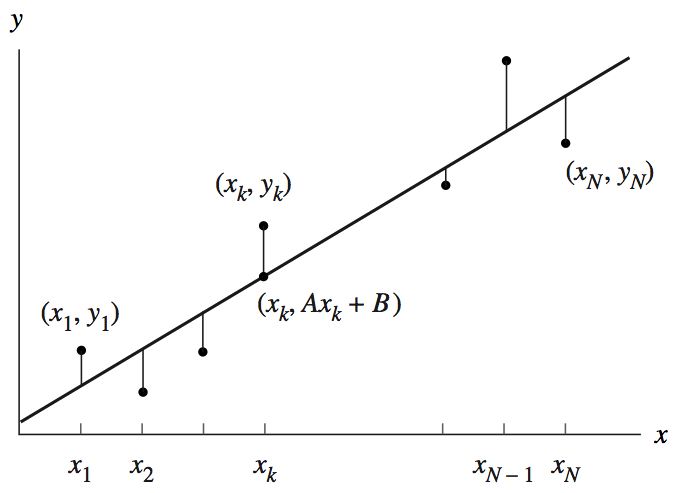
\includegraphics[width=100mm]{fig/ch-5/fig_5-2.png}
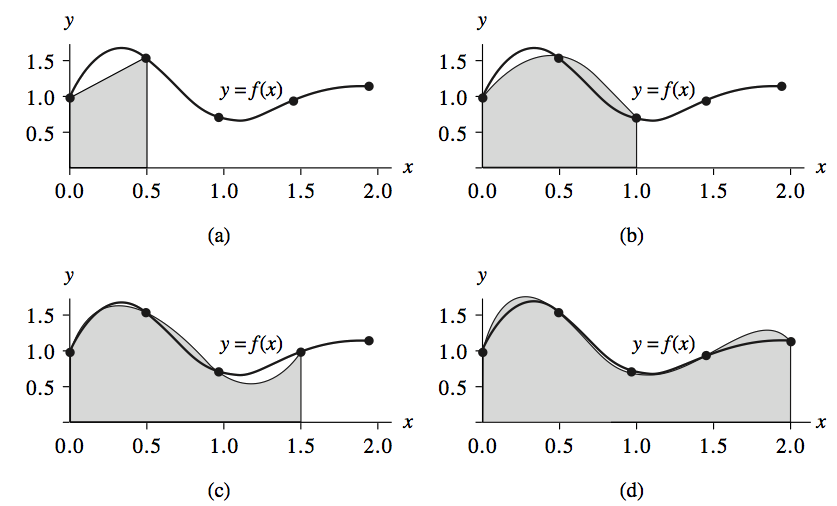
\includegraphics[width=100mm]{chap-5/fig_7-2.png}
\end{center}
\end{figure}
}




%\frame{
%\begin{itemize}
%\item In Example 5.1 we applied the quadrature rules with $h = 0.5$. 
%\item if the endpoints of the interval $[a, b]$ are held fixed, the step size must be adjusted for each rule. 
%\item The step sizes are $h = b - a$, $h = (b - a)/2$, $h = (b - a)/3$, and $h = (b - a)/4$ for the trapezoidal rule, Simpson's rule, Simpson's $\frac{3}{8}$ rule, and Boole's rule, respectively. 
%\item The next example illustrates this point. 
%\end{itemize}
%}

%\frame{
%\begin{figure}
%\begin{center}
%\includegraphics[width=110mm]{fig/ch-5/ex_5-2.png}
%\end{center}
%\end{figure}
%}

%\frame{
%\begin{figure}
%\begin{center}
%\includegraphics[width=110mm]{fig/ch-5/ex_5-2_2.png}
%\end{center}
%\end{figure}
%}

%\frame{
%\begin{figure}
%\begin{center}
%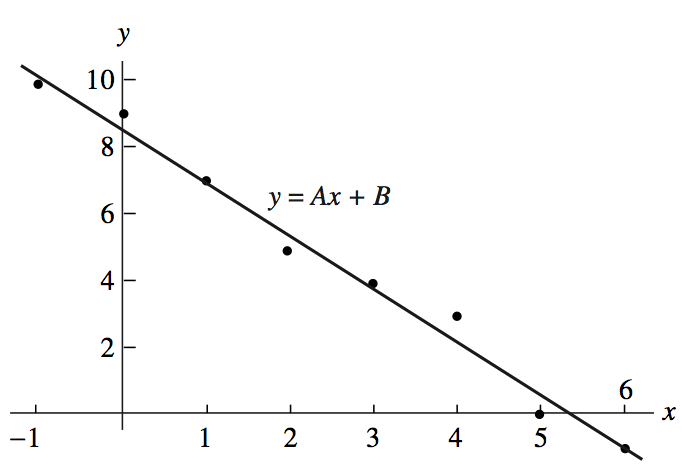
\includegraphics[width=90mm]{fig/ch-5/fig_5-3.png}
%\end{center}
%\end{figure}
%}

%\frame{
%\begin{itemize}
%\item To make a fair comparison of quadrature methods, we must use the same number of function evaluations in each method. 
%\item Our final example is concerned with comparing integration over a fixed interval $[ a, b ]$ using exactly five function evaluations $f_k = f(x_k)$, for $k = 0, 1, \ldots, 4$ for each method. 
%\item When the trapezoidal rule is applied on the four  subintervals $[ x_0, x_1 ]$, $[ x_1, x_2 ]$, $[ x_2, x_3 ]$, and $[ x_3, x_4 ]$, it is called a {\Large composite trapezoidal rule}: 
%\end{itemize}
%\begin{figure}
%\begin{center}
%\includegraphics[width=110mm]{fig/ch-5/eq_5-17.png}
%\end{center}
%\end{figure}
%}

%\frame{
%Simpson's rule can also be used in this manner. 
%When Simpson's rule is applied on the two subintervals $[ x_0, x_2 ]$ and $[ x_2, x_4 ]$, it is called a composite Simpson's rule: 
%\begin{figure}
%\begin{center}
%\includegraphics[width=90mm]{fig/ch-5/eq_5-18.png}
%\end{center}
%\end{figure}
%The next example compares the values obtained with (5.17), (5.18), and (5.7).
%}

%\frame{
%\begin{figure}
%\begin{center}
%\includegraphics[width=110mm]{fig/ch-5/ex_5-3.png}
%\end{center}
%\end{figure}
%}

%\frame{
%\begin{figure}
%\begin{center}
%\includegraphics[width=110mm]{fig/ch-5/ex_5-3_2.png}
%\end{center}
%\end{figure}
%and the approximation $1.30938$ from Simpson's rule is much better than the value $1.28358$ obtained from the trapezoidal rule. 
%\begin{itemize}
%\item Again, the approximation $1.30859$ from Boole's rule is closest. 
%\item Graphs for the areas under the trapezoids and parabolas are shown in Figure 5.4(a) and (b), respectively. 
%\end{itemize}
%}

%\frame{
%\begin{figure}
%\begin{center}
%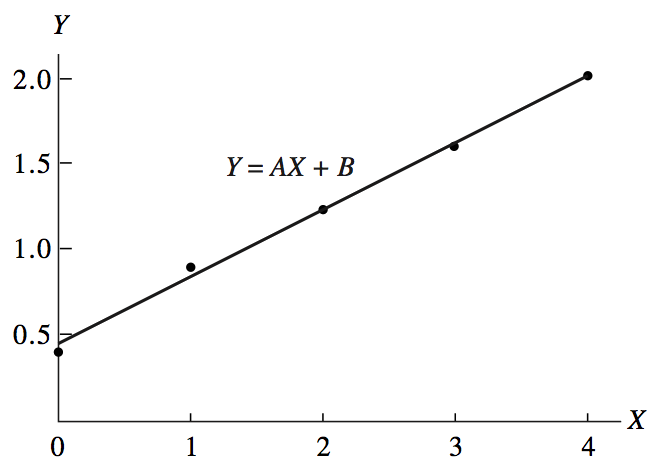
\includegraphics[width=100mm]{fig/ch-5/fig_5-4.png}
%\end{center}
%\end{figure}
%}

%\frame{
%\begin{figure}
%\begin{center}
%\includegraphics[width=110mm]{fig/ch-5/ex_5-4.png}
%\end{center}
%\end{figure}
%Therefore, the degree of precision of Simpson's $\frac{3}{8}$ rule is $n = 3$. 
%}
